% Options for packages loaded elsewhere
\PassOptionsToPackage{unicode}{hyperref}
\PassOptionsToPackage{hyphens}{url}
%
\documentclass[
]{article}
\usepackage{amsmath,amssymb}
\usepackage{lmodern}
\usepackage{iftex}
\ifPDFTeX
  \usepackage[T1]{fontenc}
  \usepackage[utf8]{inputenc}
  \usepackage{textcomp} % provide euro and other symbols
\else % if luatex or xetex
  \usepackage{unicode-math}
  \defaultfontfeatures{Scale=MatchLowercase}
  \defaultfontfeatures[\rmfamily]{Ligatures=TeX,Scale=1}
\fi
% Use upquote if available, for straight quotes in verbatim environments
\IfFileExists{upquote.sty}{\usepackage{upquote}}{}
\IfFileExists{microtype.sty}{% use microtype if available
  \usepackage[]{microtype}
  \UseMicrotypeSet[protrusion]{basicmath} % disable protrusion for tt fonts
}{}
\makeatletter
\@ifundefined{KOMAClassName}{% if non-KOMA class
  \IfFileExists{parskip.sty}{%
    \usepackage{parskip}
  }{% else
    \setlength{\parindent}{0pt}
    \setlength{\parskip}{6pt plus 2pt minus 1pt}}
}{% if KOMA class
  \KOMAoptions{parskip=half}}
\makeatother
\usepackage{xcolor}
\IfFileExists{xurl.sty}{\usepackage{xurl}}{} % add URL line breaks if available
\IfFileExists{bookmark.sty}{\usepackage{bookmark}}{\usepackage{hyperref}}
\hypersetup{
  pdftitle={Question 7: Portfolio Construction},
  pdfauthor={Andrew Hyde},
  hidelinks,
  pdfcreator={LaTeX via pandoc}}
\urlstyle{same} % disable monospaced font for URLs
\usepackage[margin=1in]{geometry}
\usepackage{color}
\usepackage{fancyvrb}
\newcommand{\VerbBar}{|}
\newcommand{\VERB}{\Verb[commandchars=\\\{\}]}
\DefineVerbatimEnvironment{Highlighting}{Verbatim}{commandchars=\\\{\}}
% Add ',fontsize=\small' for more characters per line
\usepackage{framed}
\definecolor{shadecolor}{RGB}{248,248,248}
\newenvironment{Shaded}{\begin{snugshade}}{\end{snugshade}}
\newcommand{\AlertTok}[1]{\textcolor[rgb]{0.94,0.16,0.16}{#1}}
\newcommand{\AnnotationTok}[1]{\textcolor[rgb]{0.56,0.35,0.01}{\textbf{\textit{#1}}}}
\newcommand{\AttributeTok}[1]{\textcolor[rgb]{0.77,0.63,0.00}{#1}}
\newcommand{\BaseNTok}[1]{\textcolor[rgb]{0.00,0.00,0.81}{#1}}
\newcommand{\BuiltInTok}[1]{#1}
\newcommand{\CharTok}[1]{\textcolor[rgb]{0.31,0.60,0.02}{#1}}
\newcommand{\CommentTok}[1]{\textcolor[rgb]{0.56,0.35,0.01}{\textit{#1}}}
\newcommand{\CommentVarTok}[1]{\textcolor[rgb]{0.56,0.35,0.01}{\textbf{\textit{#1}}}}
\newcommand{\ConstantTok}[1]{\textcolor[rgb]{0.00,0.00,0.00}{#1}}
\newcommand{\ControlFlowTok}[1]{\textcolor[rgb]{0.13,0.29,0.53}{\textbf{#1}}}
\newcommand{\DataTypeTok}[1]{\textcolor[rgb]{0.13,0.29,0.53}{#1}}
\newcommand{\DecValTok}[1]{\textcolor[rgb]{0.00,0.00,0.81}{#1}}
\newcommand{\DocumentationTok}[1]{\textcolor[rgb]{0.56,0.35,0.01}{\textbf{\textit{#1}}}}
\newcommand{\ErrorTok}[1]{\textcolor[rgb]{0.64,0.00,0.00}{\textbf{#1}}}
\newcommand{\ExtensionTok}[1]{#1}
\newcommand{\FloatTok}[1]{\textcolor[rgb]{0.00,0.00,0.81}{#1}}
\newcommand{\FunctionTok}[1]{\textcolor[rgb]{0.00,0.00,0.00}{#1}}
\newcommand{\ImportTok}[1]{#1}
\newcommand{\InformationTok}[1]{\textcolor[rgb]{0.56,0.35,0.01}{\textbf{\textit{#1}}}}
\newcommand{\KeywordTok}[1]{\textcolor[rgb]{0.13,0.29,0.53}{\textbf{#1}}}
\newcommand{\NormalTok}[1]{#1}
\newcommand{\OperatorTok}[1]{\textcolor[rgb]{0.81,0.36,0.00}{\textbf{#1}}}
\newcommand{\OtherTok}[1]{\textcolor[rgb]{0.56,0.35,0.01}{#1}}
\newcommand{\PreprocessorTok}[1]{\textcolor[rgb]{0.56,0.35,0.01}{\textit{#1}}}
\newcommand{\RegionMarkerTok}[1]{#1}
\newcommand{\SpecialCharTok}[1]{\textcolor[rgb]{0.00,0.00,0.00}{#1}}
\newcommand{\SpecialStringTok}[1]{\textcolor[rgb]{0.31,0.60,0.02}{#1}}
\newcommand{\StringTok}[1]{\textcolor[rgb]{0.31,0.60,0.02}{#1}}
\newcommand{\VariableTok}[1]{\textcolor[rgb]{0.00,0.00,0.00}{#1}}
\newcommand{\VerbatimStringTok}[1]{\textcolor[rgb]{0.31,0.60,0.02}{#1}}
\newcommand{\WarningTok}[1]{\textcolor[rgb]{0.56,0.35,0.01}{\textbf{\textit{#1}}}}
\usepackage{graphicx}
\makeatletter
\def\maxwidth{\ifdim\Gin@nat@width>\linewidth\linewidth\else\Gin@nat@width\fi}
\def\maxheight{\ifdim\Gin@nat@height>\textheight\textheight\else\Gin@nat@height\fi}
\makeatother
% Scale images if necessary, so that they will not overflow the page
% margins by default, and it is still possible to overwrite the defaults
% using explicit options in \includegraphics[width, height, ...]{}
\setkeys{Gin}{width=\maxwidth,height=\maxheight,keepaspectratio}
% Set default figure placement to htbp
\makeatletter
\def\fps@figure{htbp}
\makeatother
\setlength{\emergencystretch}{3em} % prevent overfull lines
\providecommand{\tightlist}{%
  \setlength{\itemsep}{0pt}\setlength{\parskip}{0pt}}
\setcounter{secnumdepth}{-\maxdimen} % remove section numbering
\ifLuaTeX
  \usepackage{selnolig}  % disable illegal ligatures
\fi

\title{Question 7: Portfolio Construction}
\author{Andrew Hyde}
\date{2022-11-26}

\begin{document}
\maketitle

\begin{Shaded}
\begin{Highlighting}[]
\NormalTok{knitr}\SpecialCharTok{::}\NormalTok{opts\_chunk}\SpecialCharTok{$}\FunctionTok{set}\NormalTok{(}\AttributeTok{echo =} \ConstantTok{FALSE}\NormalTok{, }\AttributeTok{message =} \ConstantTok{FALSE}\NormalTok{, }\AttributeTok{warning =} \ConstantTok{FALSE}\NormalTok{,}
                      \AttributeTok{fig.width =} \DecValTok{6}\NormalTok{, }\AttributeTok{fig.height =} \DecValTok{5}\NormalTok{, }\AttributeTok{fig.pos=}\StringTok{"H"}\NormalTok{, }\AttributeTok{fig.pos =}\StringTok{\textquotesingle{}H\textquotesingle{}}\NormalTok{)}
\CommentTok{\# Note: Include = FALSE implies the code is executed, but not printed in your pdf.}
\CommentTok{\# warning and message = FALSE implies ugly messages and warnings are removed from your pdf.}
\CommentTok{\# These should be picked up when you execute the command chunks (code sections below) in your rmd, not printed in your paper!}


\CommentTok{\# load packages}
\NormalTok{pacman}\SpecialCharTok{::}\FunctionTok{p\_load}\NormalTok{(}\StringTok{"tidyverse"}\NormalTok{, }\StringTok{"devtools"}\NormalTok{, }\StringTok{"rugarch"}\NormalTok{, }\StringTok{"rmgarch"}\NormalTok{, }
    \StringTok{"forecast"}\NormalTok{, }\StringTok{"tbl2xts"}\NormalTok{, }\StringTok{"lubridate"}\NormalTok{, }\StringTok{"PerformanceAnalytics"}\NormalTok{, }
    \StringTok{"ggthemes"}\NormalTok{, }\StringTok{"ks"}\NormalTok{)}
\FunctionTok{library}\NormalTok{(PortfolioAnalytics)}
\end{Highlighting}
\end{Shaded}

\begin{verbatim}
## Warning: package 'PortfolioAnalytics' was built under R version 4.2.2
\end{verbatim}

\begin{verbatim}
## Loading required package: foreach
\end{verbatim}

\begin{verbatim}
## 
## Attaching package: 'foreach'
\end{verbatim}

\begin{verbatim}
## The following objects are masked from 'package:purrr':
## 
##     accumulate, when
\end{verbatim}

\begin{Shaded}
\begin{Highlighting}[]
\FunctionTok{library}\NormalTok{(TTR)}
\NormalTok{pacman}\SpecialCharTok{::}\FunctionTok{p\_load}\NormalTok{(}\StringTok{"DEoptim"}\NormalTok{, }\StringTok{"ROI"}\NormalTok{, }\StringTok{"ROI.plugin.glpk"}\NormalTok{, }\StringTok{"ROI.plugin.quadprog"}\NormalTok{)}


\CommentTok{\# load functions}
\FunctionTok{list.files}\NormalTok{(}\StringTok{\textquotesingle{}code/\textquotesingle{}}\NormalTok{, }\AttributeTok{full.names =}\NormalTok{ T, }\AttributeTok{recursive =}\NormalTok{ T) }\SpecialCharTok{\%\textgreater{}\%}
\NormalTok{    .[}\FunctionTok{grepl}\NormalTok{(}\StringTok{\textquotesingle{}.R\textquotesingle{}}\NormalTok{, .)] }\SpecialCharTok{\%\textgreater{}\%} \FunctionTok{as.list}\NormalTok{() }\SpecialCharTok{\%\textgreater{}\%} \FunctionTok{walk}\NormalTok{(}\SpecialCharTok{\textasciitilde{}}\FunctionTok{source}\NormalTok{(.))}


\CommentTok{\# load data, and see how this can be stored and later called from your \textquotesingle{}data\textquotesingle{} folder.}
\NormalTok{MAA }\OtherTok{\textless{}{-}} \FunctionTok{read\_rds}\NormalTok{(}\StringTok{"data/MAA.rds"}\NormalTok{)}
\NormalTok{MAA}\SpecialCharTok{$}\NormalTok{Ticker }\OtherTok{\textless{}{-}} \FunctionTok{gsub}\NormalTok{(}\StringTok{" Index"}\NormalTok{, }\StringTok{""}\NormalTok{, MAA}\SpecialCharTok{$}\NormalTok{Ticker)}
\NormalTok{msci }\OtherTok{\textless{}{-}} \FunctionTok{read\_rds}\NormalTok{(}\StringTok{"data/msci.rds"}\NormalTok{) }\SpecialCharTok{\%\textgreater{}\%}
    \FunctionTok{filter}\NormalTok{(Name }\SpecialCharTok{\%in\%} \FunctionTok{c}\NormalTok{(}\StringTok{"MSCI\_ACWI"}\NormalTok{, }\StringTok{"MSCI\_USA"}\NormalTok{, }\StringTok{"MSCI\_RE"}\NormalTok{, }\StringTok{"MSCI\_Jap"}\NormalTok{))}
\end{Highlighting}
\end{Shaded}

\hypertarget{introduction}{%
\section{Introduction}\label{introduction}}

To construct the portfolio using the PortfolioAnalytics package. I take
into consideration the constraints on and requirements of the portfolio.
I follow the vignette called `Introduction to PortfolioAnalytics' by
Ross Bennett, one of the package authors, and the package documentation
to optimize this portfolio.

\hypertarget{data}{%
\section{Data}\label{data}}

I then use the `TTR' package to calculate returns for the combined data
and filter the data for the last 20 years. I pad the data by looking
back a maximum of 5 days to fill in missing values, this adds to ensure
that each asset included has at least 3 years' of returns data.

I begin by join the two data sets and select tickers in order of asset
class.

Col 1-3: Equity Col 4-5: Currency col 6-11: Bonds and Credit Col 12:
Commodity

\hypertarget{creating-the-portfolio-object}{%
\section{Creating the Portfolio
Object}\label{creating-the-portfolio-object}}

I optimize each portfolio subject to the constraints below.

Requirements: Long-only strategy When using covariance and mean
forecasts, use a look-back of less than 3 years Do not hold any assets
with less than 3 years' returns data Apply Quarterly Re-balancing Limit
exposure to Bonds and credit instruments at 25\% Limit exposure to
Equities at 60\% Limit single asset exposure at 40\%

\hypertarget{setting-up-the-porfolio}{%
\section{Setting up the porfolio}\label{setting-up-the-porfolio}}

Initially I use the random sample method to optimize the portfolio.
However, this produced different results each time the same code was
run, even after using `set.seed()'. I then opted for the ROI
optimization method to solve each portfolio.

I create three different portfolios, the first two subject to asset
exposure constraints and the last without asset exposure constraints. I
proceed to run optimization on the four portfolios to Minimize Risk,
Maximize Return and then Minimize Riks without constraints. All
positions in each portfolio is long only and all funds are invested (no
cash holdings). Each portfolio is re-balance quartely and makes use of a
rolling window = 90 days periods to calculate annulized returns.

\hypertarget{minimize-risk}{%
\section{Minimize Risk}\label{minimize-risk}}

\begin{verbatim}
## **************************************************
## PortfolioAnalytics Optimization with Rebalancing
## **************************************************
## 
## Call:
## optimize.portfolio.rebalancing(R = q7_returns_data, portfolio = minrisk, 
##     optimize_method = "ROI", search_size = 100, trace = T, rp = NULL, 
##     rebalance_on = "quarters", training_period = NULL, rolling_window = 90)
## 
## Number of rebalancing dates:  76 
## First rebalance date:
## [1] "2003-03-31"
## Last rebalance date:
## [1] "2021-10-29"
## 
## Annualized Portfolio Rebalancing Return:
## [1] 0.01668808
## 
## Annualized Portfolio Standard Deviation:
## [1] 0.022795
\end{verbatim}

\hypertarget{maximise-return}{%
\section{Maximise Return}\label{maximise-return}}

\begin{verbatim}
## **************************************************
## PortfolioAnalytics Optimization with Rebalancing
## **************************************************
## 
## Call:
## optimize.portfolio.rebalancing(R = q7_returns_data, portfolio = maxret, 
##     optimize_method = "ROI", search_size = 100, trace = T, rp = NULL, 
##     rebalance_on = "quarters", training_period = NULL, rolling_window = 90)
## 
## Number of rebalancing dates:  76 
## First rebalance date:
## [1] "2003-03-31"
## Last rebalance date:
## [1] "2021-10-29"
## 
## Annualized Portfolio Rebalancing Return:
## [1] 0.06223531
## 
## Annualized Portfolio Standard Deviation:
## [1] 0.1020928
\end{verbatim}

\hypertarget{minimize-risk-without-asset-exposure-constraints}{%
\section{Minimize Risk without Asset Exposure
Constraints}\label{minimize-risk-without-asset-exposure-constraints}}

\begin{verbatim}
## **************************************************
## PortfolioAnalytics Optimization with Rebalancing
## **************************************************
## 
## Call:
## optimize.portfolio.rebalancing(R = q7_returns_data, portfolio = pspec_4, 
##     optimize_method = "ROI", search_size = 100, trace = T, rp = NULL, 
##     rebalance_on = "quarters", training_period = NULL, rolling_window = 90)
## 
## Number of rebalancing dates:  76 
## First rebalance date:
## [1] "2003-03-31"
## Last rebalance date:
## [1] "2021-10-29"
## 
## Annualized Portfolio Rebalancing Return:
## [1] 0.02433584
## 
## Annualized Portfolio Standard Deviation:
## [1] 0.04374746
\end{verbatim}

\hypertarget{discussion-of-annualized-portfolio-results}{%
\section{Discussion of Annualized Portfolio
Results}\label{discussion-of-annualized-portfolio-results}}

\hypertarget{minimize-risk-1}{%
\section{Minimize Risk}\label{minimize-risk-1}}

Asset exposure constraints with the objective of minimize risk, led to
lower returns than if were to both minimize risk and maximize return,
but a similar degree of risk.

Annualized Portfolio Rebalancing Return: 0.01790729 Annualized Portfolio
Standard Deviation: 0.04286854

\hypertarget{mamimize-return}{%
\section{Mamimize Return}\label{mamimize-return}}

Asset exposure constraints with the objective of maximize return, led to
higher returns compared to any of the other portfolio objectives.
However, this type of optimization leads to a more than double increase
in the risk calculated by standard deviation.

Annualized Portfolio Rebalancing Return: 0.06223531 Annualized Portfolio
Standard Deviation: 0.1020928

\hypertarget{minimize-risk-without-asset-exposure-constraints-1}{%
\section{Minimize Risk without Asset Exposure
Constraints}\label{minimize-risk-without-asset-exposure-constraints-1}}

The portfolio with no asset exposure constraints that where I minimize
risk, provides higher returns than the same portfolio subject to
constraints but with a very similar level of risk.

Annualized Portfolio Rebalancing Return: 0.02433584 Annualized Portfolio
Standard Deviation: 0.04374746

\hypertarget{visualisation-of-portfolios}{%
\section{Visualisation of
Portfolios}\label{visualisation-of-portfolios}}

For the risk minimized and return maximized portfolios with asset
exposure constraints, the graphs below show the breakdown of weights as
they adjust over time. For the risk minimized portfolio we can see large
exposure to Asian and American currencies, this makes sense as the
currencies of the two largest trading countries by GDP would be very
stable given that many assets are Dollar denominated. Whereas the return
maximizing Portfolio is weights equities and bonds exposure more heavily
to achieve higher returns.

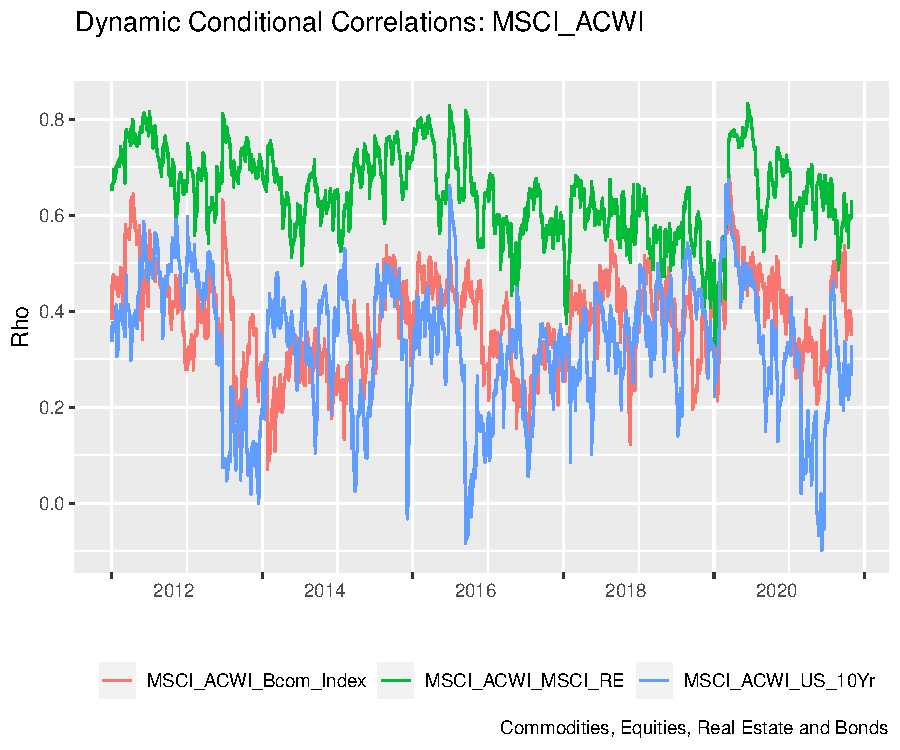
\includegraphics{Question7_files/figure-latex/unnamed-chunk-6-1.pdf}

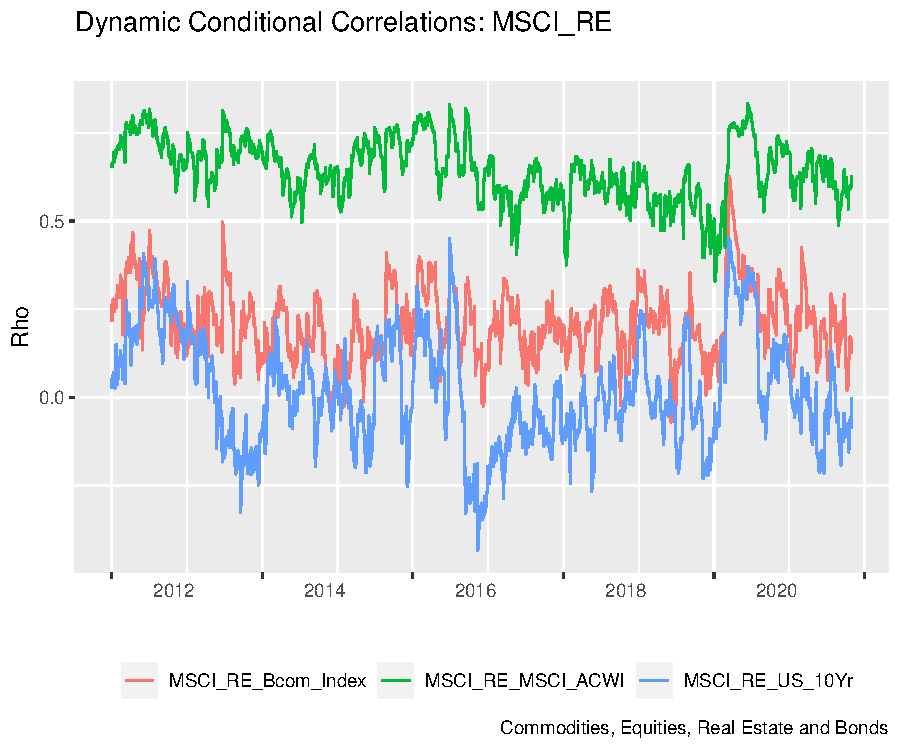
\includegraphics{Question7_files/figure-latex/unnamed-chunk-7-1.pdf}

\end{document}
